\documentclass{article}

%% Page Margins %%
\usepackage{geometry}
\geometry{
    top = 0.75in,
    bottom = 0.75in,
    right = 0.75in,
    left = 0.75in,
}

\usepackage{amsmath}
\usepackage{graphicx}
\usepackage{parskip}

\title{Assembly Project: Dr Mario}

% TODO: Enter your name
\author{Maximilian Djaya}

\begin{document}
\maketitle

\section{Instruction and Summary}

\begin{enumerate}

    \item Which milestones were implemented?
    
    Milestones 1 and 2, with 3 partly done. Just not clearing rows and columns yet.
    \item How to view the game:
    % TODO: specify the pixes/unit, width and height of 
    %       your game, etc.  NOTE: list these details in
    %       the header of your breakout.asm file too!
    
    \begin{enumerate}

    \item Open DrMario.asm in MARS.
    \item Open the bitmap.
    \begin{enumerate}
        \item set the pixel height to 8
        \item set the pixel width to 8
        \item set the display width to 512
        \item set the display height to 512
        \item change the base address to 0x10008000
        \item click connect to MIPS.
    \end{enumerate}
    \item Open the keyboard input and click connect to MIPS.
    \item Assemble DrMario.asm and run.


    \end{enumerate}

    

\begin{figure}[ht!]
    \centering
    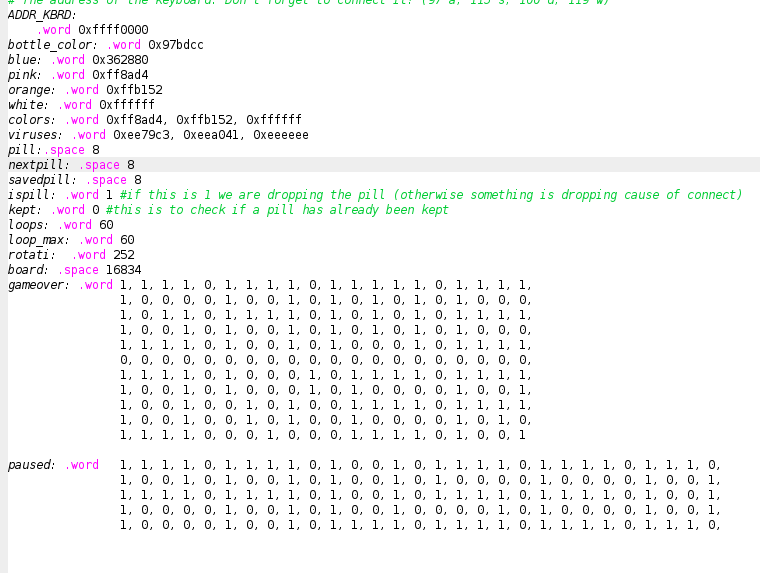
\includegraphics[width=0.3\textwidth]{memory.png}
    \caption{What memory is initialized to}
    \label{Instructions}
\end{figure}

\item Game Summary:
\begin{itemize}
\item It is just dr mario so far. (WASD to move)
\item Each second your pill falls one row
\item When the pill collides with something below it a new pill spawns
\item Press C to save the pill for later or retrieve a saved pill
\item There are all the previewed capsules in the side jar on the right
\item Press p to pause the game
\item When you get 4 or more in a row those capsules clear
\item Then any unsupported capsule drops
\item When the entrance is blocked Game Over happens
\item Press r to restart the game if you've reached game over
\item Each time rows clear, the gravity speeds up
\item There are sound effects
\end{itemize}
\item Features
\begin{itemize}
\item Easy: Gravity
\item Easy: Speed up gravity as you clear rows
\item Easy: Sound Effects
\item Easy: Game Over
\item Easy: Pause
\item Easy: Save Capsule
\item Easy: Preview 1 capsule
\item Easy: Preview 4-5 capsules
\end{itemize}

    
\end{enumerate}

\section{Attribution Table}
% TODO: If you worked in partners, tell us who was 
%       responsible for which features. Some reweighting 
%       might be possible in cases where one group member
%       deserves extra credit for the work they put in.

\begin{center}
\begin{tabular}{|| c ||}
\hline
 Maximilian Djaya (1010401744)\\ 
 \hline
 Everything
\end{tabular}
\end{center}

% TODO: Fill out the remainder of the document as you see 
%       fit, including as much detail as you think 
%       necessary to better understand your code. 
%       You can add extra sections and subsections to 
%       help us understand why you deserve marks for 
%       features that were more challenging than they
%       might initially seem.

\begin{enumerate}
    \item Milestone 1
    
    Fairly easy, just used a drawline function to draw the bottle and drawpill function with random syscall to make pills. Then just more random calls for the viruses.
    \item Milestone 2
    
    Pretty easy too, just used a couple functions to respond to movement
    \item Milestone 3
    
    HARD, Collision detection was pretty easy and so was clearing rows,
    but I had to consider how to implement dropping unsupported capsules so that the logic is the same as the original game. I had to add an array where I keep the location of the other half of pills. And had to consider cases where the other half gets destroyed. Then I still had to make sure they dropped properly.
    
    \item Milestones 4-5
    
    All the features that I implemented were fairly easy - medium difficult, so I don't think I should get any extra points here
\end{enumerate}

\end{document}